\documentclass[11pt]{article}
\usepackage[T1]{fontenc}
\usepackage[utf8]{inputenc}
\usepackage{lmodern,microtype}
\usepackage[margin=1in]{geometry}
\usepackage{amsmath,amssymb,amsthm,mathtools}
\usepackage{booktabs,longtable,array,graphicx,xcolor,enumitem}
\usepackage{xurl}
\usepackage[colorlinks=true,linkcolor=blue!55!black,citecolor=blue!55!black,urlcolor=blue!55!black]{hyperref}
\usepackage[nameinlink,noabbrev]{cleveref}
\usepackage{fancyhdr}
\pagestyle{fancy}\fancyhf{}
\fancyhead[L]{Symplectic cycle dependence}\fancyhead[R]{Research report}
\fancyfoot[C]{\thepage}
\setlength{\headheight}{14pt}
\setlength{\emergencystretch}{2em}
\newtheorem{theorem}{Theorem}[section]
\newtheorem{proposition}[theorem]{Proposition}
\newtheorem{lemma}[theorem]{Lemma}
\newtheorem{corollary}[theorem]{Corollary}
\theoremstyle{definition}\newtheorem{definition}[theorem]{Definition}
\theoremstyle{remark}\newtheorem{remark}[theorem]{Remark}
\newcommand{\F}{\mathbb F}
\newcommand{\E}{\mathbb E}
\newcommand{\Prob}{\mathbb P}
\newcommand{\TV}{d_{\mathrm{TV}}}
\newcommand{\KL}{D_{\mathrm{KL}}}
\newcommand{\one}{\mathbf1}
\newcommand{\Sp}{\operatorname{Sp}}
\newcommand{\rank}{\operatorname{rank}}
\newcommand{\tr}{\operatorname{tr}}
\newcommand{\Var}{\operatorname{Var}}
\newcommand{\supp}{\operatorname{supp}}
\newcommand{\abs}[1]{\lvert#1\rvert}
\newcommand{\norm}[1]{\lVert#1\rVert}
\newcommand{\pair}[2]{\langle#1,#2\rangle}
\title{\textbf{Exact cycle dependence and sharp detection\\in finite symplectic observations}\\[5pt]
\large An extension of the finite-field methods in the ProveIt GRH program}
\author{Prepared for Vladimir Reshetnikov}
\date{27 November 2026}
\hypersetup{pdftitle={Exact cycle dependence and sharp detection in finite symplectic observations},pdfauthor={Research report prepared for Vladimir Reshetnikov},pdfsubject={Finite fields, exact cycle laws, cactus testing profiles, and overlapping-cycle counterexamples}}
\begin{document}
\maketitle
\begin{abstract}
Choose independent nonzero vectors in a finite symplectic space and reveal their
pairings along the edges of a graph. We determine the complete joint law on every
cycle, in every characteristic. On forests the edge observations are exactly
independent, and independence holds only on forests. For cactus graphs, even cycles
sharing vertices contribute independent blocks. Exact total variation and
chi-square formulas reveal a parity phenomenon: cycles of lengths $2r+1$ and
$2r+2$ carry the same leading information,
$(q-1)^{2r+1}q^{-4nr}$, in ambient dimension $2n$.

For arbitrary growing cactus graphs with bounded cycle lengths, we prove a sharp
testing theorem. If the sum of the cycle chi-square divergences tends to
$\tau\in[0,\infty)$, the total variation distance from independent edges tends to
$2\Phi(\sqrt{\tau}/2)-1$; if that sum diverges, the distance tends to one.
This determines the critical window, the optimal testing error, and simple
asymptotically optimal statistics. Over $\F_2$, cycle parities suffice. A
complete-bipartite contrast shows why adding the signals of overlapping cycles
can predict the wrong threshold by an exponential factor.

The results are unconditional. Their connection with the supplied repository is
the finite-field Fourier and symplectic counting mechanism. We give complete
proofs and reproducible exact-arithmetic checks. Novelty is assessed against a
pinned repository snapshot and specified related literature; worldwide priority
and Lean formalization are not asserted.
\end{abstract}
\tableofcontents
\section{Main result and mathematical context}\label{sec:intro}

\subsection{A concrete phenomenon}
Fix a finite field $\F_q$, an integer $n\ge1$, a nondegenerate alternating bilinear form on
$V=\F_q^{2n}$, and a finite simple graph $G$. At each vertex $v$, independently
choose a uniform nonzero vector $X_v$. An oriented edge $u\to v$ reveals
\[
Y_{uv}=\pair{X_u}{X_v}.
\]
Repeated vectors at different vertices are allowed. We compare these observations
with independent field elements having exactly the same one-edge distribution.

A tree reveals no dependence at all, regardless of its size. A cycle reveals
dependence only when all of its edges are retained: the joint law of any proper
subset of its edges is exactly the independent law. Nevertheless, enough complete
cycles permit nearly certain detection of the hidden common geometry. The number
required grows exponentially in the ambient dimension, and adding one edge to an
odd cycle does not change its leading information.

These statements concern the entire labelled edge vector. They are stronger than
a count of configurations with one specified label. The comparison retains
the true one-edge bias. Comparing instead with independent uniform labels would
introduce an additional signal already visible on single edges.

\begin{figure}[htbp]
\centering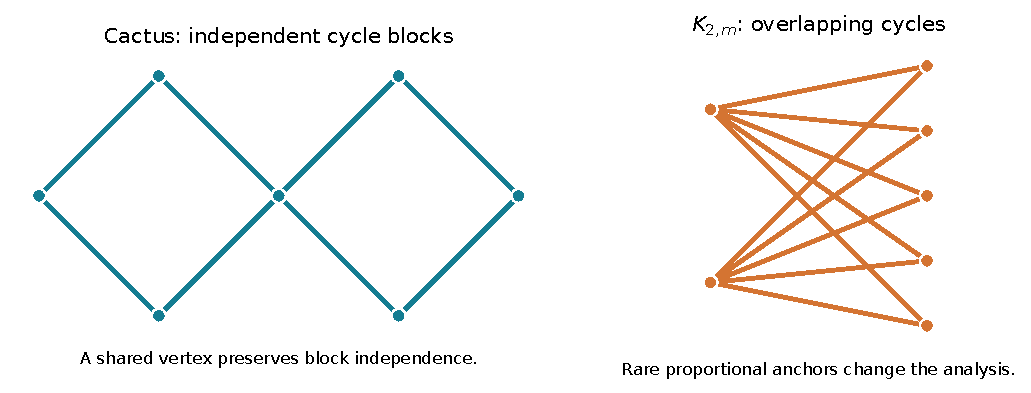
\includegraphics[width=.96\linewidth]{figures/observation_graphs.pdf}
\caption{Two observation patterns. Cycle blocks in a cactus are independent even when they share a vertex. Complete bipartite observations have overlapping cycles and a different detection calculation.}
\end{figure}

\subsection{The sharp detection theorem}
Put $N=q^{2n}$. For $\ell\ge3$ define
\begin{equation}\label{eq:info}
v_{\ell,N}=
\begin{cases}
\displaystyle (q-1)^\ell\frac{N}{(N-q)^\ell},&\ell\text{ odd},\\[7pt]
\displaystyle (q-1)^{\ell-2}
\bigl((N-q)^{2-\ell}+(q-2)(N-1)^{2-\ell}\bigr),&\ell\text{ even}.
\end{cases}
\end{equation}
A \emph{cactus} is a finite simple graph in which two distinct simple cycles
have at most one common vertex. Trees, disjoint unions of cycles, and arbitrarily
many cycles attached at one common vertex are examples.

\begin{theorem}[Sharp detection on growing cactus graphs]\label{thm:main}
Fix $q$ and an integer $L\ge3$. For each $n$, let $G_n$ be any cactus graph whose
cycle lengths belong to $\{3,\ldots,L\}$. The graph may have arbitrarily many
vertices and bridges. Let $P_n$ be its symplectic edge law and $Q_n$ the product
of its true one-edge marginals. Let $\mathcal C_n$ be its set of cycles and put
\[
I_n=\sum_{C\in\mathcal C_n}v_{|C|,q^{2n}}.
\]
Then:
\begin{enumerate}[label=(\roman*)]
\item If $I_n\to\tau\in[0,\infty)$, then
\begin{equation}\label{eq:profile}
\TV(P_n,Q_n)\longrightarrow 2\Phi(\sqrt{\tau}/2)-1,
\end{equation}
where $\Phi$ is the standard normal distribution function.
\item If $I_n\to\infty$, then $\TV(P_n,Q_n)\to1$.
\item If $0<\tau<\infty$, the log likelihood ratio converges in distribution to
$\mathcal N(-\tau/2,\tau)$ under $Q_n$ and to
$\mathcal N(\tau/2,\tau)$ under $P_n$. The minimum average error with equal prior
probabilities tends to $\Phi(-\sqrt{\tau}/2)$.
\end{enumerate}
All assertions include characteristic two.
\end{theorem}

For either of the two lengths $\ell=2r+1$ and $\ell=2r+2$,
\begin{equation}\label{eq:pair}
v_{\ell,N}=(q-1)^{2r+1}N^{-2r}(1+O_{q,r}(N^{-1})).
\end{equation}
Consequently, if a cactus has $m_n$ cycles, all of either one of these lengths
or any mixture of the two, its critical scale is
\begin{equation}\label{eq:critical}
m_n\asymp\frac{q^{4nr}}{(q-1)^{2r+1}}.
\end{equation}
More precisely, $m_n(q-1)^{2r+1}q^{-4nr}\to\tau$ gives
\eqref{eq:profile}. This is an equality of leading statistical information;
the two finite-dimensional laws need not coincide.

\subsection{What is inherited and what is added}
The supplied repository was inspected at commit
\texttt{00cadb961bbe77c74e5d082c4948f8884d58a970}.
Its merged article contains finite-field Fourier estimates, positive-type
stabilizer bounds, exact laws for two arbitrary symplectic frames, and numerous
rank and residual-form comparisons \cite{ProveItSpn}. In particular,
\texttt{spn:lem:alt-gram} evaluates Fourier coefficients of a random alternating
Gram matrix by the rank of the Fourier variable. The transfer from the original
proof program to finite-field statistics is also described in its source
section \cite{ProveItSrc}.

Several apparently natural extensions are already covered by current Research
packets: fixed-gap rectangular blocks, exact two-frame tests, and joint
rank/defect expansions \cite{ProveItTwo,ProveItRect}. We do not claim these.
Earlier work in the same research program also supplied a several-frame
threshold and forest independence. We take the forest observation as a starting
point and prove it again for self-containment.

The additions here are the full labelled cycle laws, their exact information and
distance formulas, the even-cycle resonance, the equality \eqref{eq:pair}, the
sharp growing-cactus testing theorem, and a contrasting overlapping-cycle family.
Classical symplectic graph spectra and finite-field cycle counts are adjacent
subjects \cite{TangWan,IJM,Bright}; individual fixed-label counts and the Fourier
technique alone are not presented as new. The broader question of
observation-graph-dependent detectability also has an established counterpart
for real Wishart models \cite{BBH}. Our statements specify an exact finite-field
experiment and its explicit critical profile. The novelty assessment is scoped
in \cref{sec:provenance}.


\section{Exact cycle laws for symplectic edge observations}\label{sec:cycles}

Let $n\ge1$ and let $V=\mathbb F_q^{2n}$ carry a nondegenerate alternating bilinear form
$\langle\ ,\ \rangle$, put $N=q^{2n}$, and let $X_v$ be independent uniform
vectors in $V\setminus\{0\}$. An oriented edge $u\to v$ records
$Y_{uv}=\langle X_u,X_v\rangle$. Its law is
\[
 p_N(a)=\begin{cases}(N-q)/(q(N-1)),&a=0,\\
 N/(q(N-1)),&a\ne0.\end{cases}
\]
All coordinates of this law are positive since $N\ge q^2$.
Reversing an edge negates its label. This coordinatewise bijection preserves
$p_N$ and the product reference law, so it preserves total variation and
chi-square divergence. Thus any fixed cycle orientation can be converted
to the cyclic orientation used below.
For a cyclically oriented cycle of length $\ell\ge3$, write $\mu_{\ell,N}$
for the edge-vector law and $\pi_{\ell,N}=p_N^{\otimes\ell}$.
Put $\kappa(0)=q-1$ and $\kappa(a)=-1$ for $a\ne0$.

\subsection{The Fourier law}\label{sec:fourier}
\begin{theorem}[Complete cycle Fourier law]\label{thm:fourier}
Fix any nontrivial additive character $\psi$ of $\mathbb F_q$ and use
$\widehat\mu(t)=\mathbb E\psi(\sum_i t_iY_i)$.
If at least one $t_i$ is zero, then
\[
 \widehat\mu_{\ell,N}(t)=\left(-\frac1{N-1}\right)^{\#\{i:t_i\ne0\}}
 =\widehat\pi_{\ell,N}(t).
\]
If all $t_i\ne0$, then
\[
 \widehat\mu_{2k+1,N}(t)=\frac{N^{k+1}-1}{(N-1)^{2k+1}},
\]
and
\[
 \widehat\mu_{2k,N}(t)=
 \frac{1+N^k\bigl((N-1){\bf1}_{t_1t_3\cdots t_{2k-1}=t_2t_4\cdots t_{2k}}-1\bigr)}
 {(N-1)^{2k}}.
\]

\end{theorem}
\begin{proof}
Forests have independent edge labels: condition on all vertices except a
leaf; its label has the same law $p_N$ for every value of its nonzero
neighbor, and remove leaves inductively. Zero Fourier coordinates remove
edges and leave a forest.
For the full cycle define matrices indexed by $V\setminus\{0\}$,
\[
 F_t(x,y)=\psi(t\langle x,y\rangle),\qquad
 P_c(x,z)={\bf1}_{z=cx},\qquad J(x,z)=1.
\]
For $t\ne0$, additive orthogonality gives $F_t\mathbf1=-\mathbf1$, and
\[
 F_sF_t=NP_{s/t}-J.
\]
The constant subspace and its orthogonal complement $H$ are invariant.
On $H$, pair the factors in the cycle trace. For an even cycle their
product is $N^kP_c$ with
$c=t_1t_3\cdots t_{2k-1}/(t_2t_4\cdots t_{2k})$.
The trace of $P_c$ on $H$ is $(N-1){\bf1}_{c=1}-1$.
For an odd cycle the product is $N^kP_cF_t$ on $H$.
Every diagonal entry of $P_cF_t$ is $1$, because the form is alternating,
so its full trace is $N-1$; its constant eigenvalue is $-1$, and hence
its trace on $H$ is $N$.
Adding the constant eigenvalue $(-1)^\ell$ and dividing by
$(N-1)^\ell$ proves the formulas. No division by $2$ occurs, so the proof
includes characteristic $2$.
\end{proof}

\subsection{Pointwise inversion and the even-cycle resonance}
\begin{theorem}[Exact pointwise cycle law]\label{thm:pmf}
For odd $\ell=2k+1$,
\[
 \mu_{\ell,N}(a)-\pi_{\ell,N}(a)
 =\frac{N^{k+1}}{q^\ell(N-1)^\ell}\prod_{i=1}^\ell\kappa(a_i).
\tag{O}\label{eq:odd-pmf}
\]
For even $\ell=2k$, define the integer-valued function
\[
 K_\ell(a)=
 \sum_{\substack{t_i\in\mathbb F_q^\times\\
 t_1t_3\cdots t_{\ell-1}=t_2t_4\cdots t_\ell}}
 \psi\left(-\sum_i t_ia_i\right).
\]
Then
\[
 \mu_{\ell,N}(a)-\pi_{\ell,N}(a)
 =\frac{N^k}{q^\ell(N-1)^\ell}
 \left((N-1)K_\ell(a)-\prod_i\kappa(a_i)\right).
\tag{E}\label{eq:even-pmf}
\]
The sum defining $K_\ell$ has the explicit real evaluation
\[
 K_\ell(a)=\begin{cases}
 \displaystyle\frac{\prod_i\kappa(a_i)}{q-1},
     &\text{some }a_i=0,\\[6pt]
 \displaystyle\frac{1+q^k((q-1){\bf1}_{\mathcal R(a)}-1)}{q-1},
     &\text{all }a_i\ne0,
 \end{cases}
\]
where
\[
 \mathcal R(a):\quad
 a_1a_3\cdots a_{2k-1}=(-1)^k a_2a_4\cdots a_{2k}.
\]
This is a multiplicative resonance condition on the observed edge labels.

\end{theorem}
\begin{proof}
Additive Fourier inversion gives
\[
 \mu_{\ell,N}(a)-\pi_{\ell,N}(a)
 =q^{-\ell}\sum_{t\in\mathbb F_q^\ell}
 \bigl(\widehat\mu_{\ell,N}(t)-\widehat\pi_{\ell,N}(t)\bigr)
 \psi\left(-\sum_i t_i a_i\right).
\]
By \cref{thm:fourier}, the summand vanishes whenever any $t_i=0$.
For odd $\ell$, the remaining Fourier difference is constant, and
$\sum_{t\ne0}\psi(-ta)=\kappa(a)$ gives (O).
For even $\ell$, separating the balanced-frequency indicator from the
constant term gives (E). It remains to evaluate $K_\ell$.
Insert multiplicative-character orthogonality for the constraint on $t$.
The trivial character contributes $\prod_i\kappa(a_i)/(q-1)$.
If some $a_i=0$, every nontrivial-character term vanishes.
If all $a_i\ne0$, let $G(\chi)=\sum_{x\ne0}\chi(x)\psi(x)$.
The nontrivial-character contribution factors into $k$ copies of each
Gauss sum, with
$G(\chi)G(\chi^{-1})=\chi(-1)q$.
It is therefore
\[
 \frac{q^k}{q-1}\sum_{\chi\ne1}
 \chi\left((-1)^k\frac{a_2a_4\cdots a_{2k}}{a_1a_3\cdots a_{2k-1}}\right).
\]
The last character sum is $q-2$ on $\mathcal R(a)$ and $-1$ elsewhere.
The Gauss identity follows directly by setting $x=uy$ in
$G(\chi)G(\chi^{-1})$ and summing over $y$; thus this inversion needs no
external theorem beyond finite-field character orthogonality.
\end{proof}

\subsection{Exact total variation and chi-square divergences}
\begin{theorem}[Exact one-cycle distances]\label{thm:distances}
Use
$d_{\rm TV}(\mu,\pi)=\frac12\sum_a|\mu(a)-\pi(a)|$ and
$\chi^2(\mu\Vert\pi)=\sum_a(\mu(a)-\pi(a))^2/\pi(a)$.
For odd $\ell=2k+1$,
\[
 d_{\rm TV}(\mu_{\ell,N},\pi_{\ell,N})=
 2^{\ell-1}(1-q^{-1})^\ell\frac{N^{k+1}}{(N-1)^\ell},
\tag{TV-O}
\]
\[
 \chi^2(\mu_{\ell,N}\Vert\pi_{\ell,N})
 =(q-1)^\ell\frac{N}{(N-q)^\ell}.
\tag{CS-O}
\]
For even $\ell=2k$,
\begin{align*}
 d_{\rm TV}(\mu_{\ell,N},\pi_{\ell,N})
 ={}&\frac{N^k(q-1)^{\ell-2}}{q^\ell(N-1)^\ell}\\
 &\quad\times\left[
 (N-q)\bigl((q-1)2^{\ell-1}-(q-2)\bigr)
 +(N-1)(q-2)q^k\right],
\tag{TV-E}
\end{align*}
\[
 \chi^2(\mu_{\ell,N}\Vert\pi_{\ell,N})
 =(q-1)^{\ell-2}
 \left((N-q)^{2-\ell}+(q-2)(N-1)^{2-\ell}\right).
\tag{CS-E}
\]

\end{theorem}
\begin{proof}
\textit{Odd computation.}
Equation (O) and $\sum_a|\kappa(a)|=2(q-1)$ give (TV-O).
For (CS-O), put
\[
 b_N(0)=\frac{(q-1)N}{N-q},\qquad b_N(a)=-1\ (a\ne0).
\]
Then $\mathbb E_{p_N}b_N=0$,
$\mathbb E_{p_N}b_N^2=(q-1)N/(N-q)$, and
\[
 \frac{\mu_{2k+1,N}(a)}{\pi_{2k+1,N}(a)}-1
 =N^{-k}\prod_i b_N(a_i).
\]
Squaring and factoring the expectation proves (CS-O).

\textit{Even computation.}
Write $A=N-q$, $C=(N-1)q^k$ and
$B(a)=(N-1)K_\ell(a)-\prod_i\kappa(a_i)$.
If $z\ge1$ coordinates of $a$ vanish, then
$B(a)=A\prod_i\kappa(a_i)/(q-1)$, so its sign is
$(-1)^z$ (as $\ell$ is even).
If all coordinates are nonzero, then
\[
 B(a)=\begin{cases}(A+(q-2)C)/(q-1),&\mathcal R(a),\\
 (A-C)/(q-1),&\neg\mathcal R(a).
 \end{cases}
\]
The first expression is positive and the second negative whenever its
class is nonempty. There are $(q-1)^{\ell-1}$ resonant vectors and
$(q-2)(q-1)^{\ell-1}$ nonresonant vectors.
For vectors having at least one zero coordinate, the sum of $|B|$ is
\[
 A(q-1)^{\ell-1}(2^\ell-1).
\]
The sum over vectors without zeros is
\[
 (q-1)^{\ell-2}\bigl((3-q)A+2(q-2)C\bigr).
\]
Adding these terms and multiplying by
$N^k/[2q^\ell(N-1)^\ell]$ gives (TV-E).
For chi-square, (E) gives
\[
 \chi^2=\frac1{q^\ell(N-1)^\ell}
 \sum_a\left(\frac N{N-q}\right)^zB(a)^2.
\]
The terms with $z\ge1$ sum to
\[
 (q-1)^{\ell-2}A^2
 \left[\left(\frac{q(N-1)}A\right)^\ell-1\right].
\]
The $z=0$ terms sum to
$(q-1)^{\ell-2}(A^2+(q-2)C^2)$.
The cancellation of the $A^2$ terms and $q^{2k}=q^\ell$ give (CS-E).
\end{proof}

\section{Cactus factorization and independence}\label{sec:cactus}
\begin{theorem}[Exact block independence]\label{thm:cactus}
A cactus graph is a finite simple graph whose distinct cycles have at
most one common vertex. Its blocks containing edges are bridges and simple
cycles; isolated vertices carry no observations.
Under the symplectic model, the edge vectors associated with all these
blocks are mutually independent. Each bridge has law $p_N$, and each
cyclically oriented cycle of length $\ell$ has law $\mu_{\ell,N}$.

\end{theorem}
\begin{proof}
For a block sharing an articulation vertex $v$ with the remainder,
condition on all vectors outside the block except $X_v$.
The remaining random vectors in the block are independent and uniform.
The conditional law of its edge labels given $X_v=x$ is independent of
the chosen nonzero $x$: the symplectic group acts transitively on
$V\setminus\{0\}$ and preserves all labels, while carrying uniform
vectors to uniform vectors. Hence the block labels are independent of
everything in the remaining graph. Remove leaf blocks in the block-cut
tree and iterate. The same argument works componentwise.
\end{proof}

\begin{corollary}[Independence characterizes forests]\label{cor:forest}
For any finite simple graph $G$, its edge labels are independent if and
only if $G$ is a forest.
\end{corollary}
\begin{proof}
Sufficiency was proved above. If $G$ has a cycle,
retain its cycle-edge marginal; it has one of the strictly positive TV
distances (TV-O) or (TV-E), so the complete family cannot be independent.
\end{proof}

\subsection{Paired cycle lengths}
\begin{corollary}[Equal leading information]\label{cor:paired}
For each fixed $q$ and $r\ge1$, both lengths
$\ell=2r+1$ and $\ell=2r+2$ satisfy
\[
 \chi^2(\mu_{\ell,N}\Vert\pi_{\ell,N})
 =(q-1)^{2r+1}N^{-2r}(1+O_{q,r}(N^{-1})).
\]
Moreover, uniformly in $a$,
$\mu_{\ell,N}(a)/\pi_{\ell,N}(a)-1=O_{q,\ell}(N^{-r})$.
\end{corollary}
\begin{proof}
The information asymptotics follow by expanding (CS-O) and (CS-E). In the even case the leading factor is $(q-1)^{2r}(1+q-2)=(q-1)^{2r+1}$.
The uniform likelihood bound follows at once from (O), (E), and $p_N(a)\to1/q$.
\end{proof}


\section{Proof of the sharp testing profile}\label{sec:testing}
We use
\[
\TV(P,Q)=\frac12\sum_y|P(y)-Q(y)|,\qquad
\chi^2(P\Vert Q)=\sum_y\frac{(P(y)-Q(y))^2}{Q(y)}
\]
for finite probability measures with $Q>0$. Throughout, empty products equal
$1$, empty sums equal $0$, and the maximum of an empty family of nonnegative
bounds equals $0$. In particular, these conventions include graphs with no
cycles. The factorization proved above implies
\begin{equation}\label{eq:factor}
\frac{dP_G}{dQ_G}(y)=
\prod_{C\in\mathcal C(G)}
\frac{\mu_{|C|,N}(y_C)}{\pi_{|C|,N}(y_C)},\qquad
1+\chi^2(P_G\Vert Q_G)=
\prod_{C\in\mathcal C(G)}(1+v_{|C|,N}).
\end{equation}
Bridges have identical factors in both experiments. Deleting one edge from every
cycle makes the remaining observations exactly independent.

\subsection{A product experiment lemma}
\begin{lemma}[Many small independent likelihood increments]\label{lem:lan}
For each index $n$, let $Q_n=\bigotimes_jQ_{n,j}$ and
$P_n=\bigotimes_jP_{n,j}$ be finite products. Write
\[
\frac{dP_{n,j}}{dQ_{n,j}}=1+u_{n,j},\quad
v_{n,j}=\E_{Q_{n,j}}u_{n,j}^2,\quad
I_n=\sum_jv_{n,j},\quad
\delta_n=\max_j\|u_{n,j}\|_\infty.
\]
Assume $\delta_n\to0$. Then the conclusions of \cref{thm:main} hold with these
$P_n,Q_n,I_n$.
\end{lemma}
\begin{proof}
Each $u_{n,j}$ has mean zero under $Q_{n,j}$. For $|u|\le\delta<1/2$,
Taylor's theorem gives uniform estimates
\[
\log(1+u)=u-\tfrac12u^2+O(\delta u^2),\qquad
|\log(1+u)|\le2|u|.
\]
Consequently, for $Z_n=\sum_j\log(1+u_{n,j})$,
\begin{align*}
\E_{Q_n}Z_n&=-\tfrac12 I_n+O(\delta_n I_n),\\
\Var_{Q_n}Z_n&=I_n+O(\delta_n I_n).
\end{align*}
For the variance estimate, the sum of squared individual means is
$O(\sum_jv_{n,j}^2)\le O(\delta_n^2 I_n)$.
The sum of centered third absolute moments is $O(\delta_n I_n)$.
If $I_n\to\tau\in(0,\infty)$, the Lyapunov central limit theorem gives
\[
Z_n\ \Longrightarrow\ \mathcal N(-\tau/2,\tau)
\quad\text{under }Q_n.
\]
Equivalently one can expand the characteristic functions: the error in the
quadratic approximation is bounded by the same sum of third moments.

Under $P_{n,j}$, expectations satisfy
$\E_{P_{n,j}}f=\E_{Q_{n,j}}(1+u_{n,j})f$.
The same Taylor estimates give mean $v_{n,j}/2+O(\delta_n v_{n,j})$,
variance $v_{n,j}+O(\delta_n v_{n,j})$, and identical third-moment control.
Hence $Z_n\Longrightarrow\mathcal N(\tau/2,\tau)$ under $P_n$.

For total variation use the bounded continuous function
\[
\TV(P_n,Q_n)=\E_{Q_n}(1-e^{Z_n})_+.
\]
If $Z\sim\mathcal N(-\tau/2,\tau)$, direct Gaussian integration gives
\[
\E(1-e^Z)_+
=\Prob(Z<0)-\E(e^Z\one_{\{Z<0\}})
=\Phi(\sqrt\tau/2)-\Phi(-\sqrt\tau/2).
\]
Thus this convergence step does not require a separate
uniform-integrability assumption on likelihood ratios.

If $I_n\to0$, the product identity and Cauchy--Schwarz give
\[
\TV(P_n,Q_n)\le\frac12
\sqrt{\prod_j(1+v_{n,j})-1}
\le\frac12\sqrt{e^{I_n}-1}\longrightarrow0.
\]

If $I_n\to\infty$, use the Hellinger affinity
$A_n=\E_{Q_n}\sqrt{dP_n/dQ_n}$.
For $|u|\le\delta<1$, Taylor's theorem and
$-\frac{d^2}{du^2}\sqrt{1+u}\ge1/(4(1+\delta)^{3/2})$ give
\[
\E_{Q_{n,j}}\sqrt{1+u_{n,j}}
\le1-\frac{v_{n,j}}{8(1+\delta_n)^{3/2}}.
\]
Independence implies
\[
A_n\le\exp\left(-\frac{I_n}{8(1+\delta_n)^{3/2}}\right)\longrightarrow0.
\]
Since $1-\TV(P_n,Q_n)=\sum\min(P_n,Q_n)\le A_n$, the distance tends to one.
Finally the minimum equal-prior average testing error is
$(1-\TV(P_n,Q_n))/2$.
\end{proof}

\subsection{Application and finite bounds}
\begin{proof}[Proof of \cref{thm:main}]
By \cref{thm:cactus}, discard the identical bridge factors, leaving independent
cycle factors. By \cref{thm:distances}, their variances are exactly
\eqref{eq:info}. The cycle lengths form a fixed finite set, so
\cref{cor:paired} gives $\delta_n=O_{q,L}(N^{-1})\to0$.
Apply \cref{lem:lan}.
\end{proof}

For finite parameters, if
$\delta=\max_C\|\mu_{|C|,N}/\pi_{|C|,N}-1\|_\infty<1$ and
$I=\sum_Cv_{|C|,N}$, the proof gives
\begin{equation}\label{eq:finite-bounds}
1-\exp\left(-\frac I{8(1+\delta)^{3/2}}\right)
\le\TV(P_G,Q_G)
\le\min\left\{1,\frac12\sqrt{e^I-1}\right\}.
\end{equation}
The grouped law in \cref{app:groups} computes $I$ and $\delta$ from at most
$\ell+2$ outcomes per cycle.

\begin{corollary}[Relative entropy and testing errors]\label{cor:information}
In \cref{thm:main}, whenever $I_n=O(1)$,
\[
\KL(P_n\Vert Q_n)=\tfrac12 I_n+o(1),\qquad
\KL(Q_n\Vert P_n)=\tfrac12 I_n+o(1).
\]
For sufficiently large $n$ all cycle likelihoods are strictly positive.
If $I_n\to\tau>0$, the likelihood-ratio test has both error probabilities
tending to $\Phi(-\sqrt\tau/2)$.
\end{corollary}
\begin{proof}
Use the two expectations of $Z_n$ in the proof of \cref{lem:lan}.
Strict positivity follows from $\delta_n<1$. The normal limits at threshold
$Z_n=0$ give the two error probabilities.
\end{proof}

\section{Simple optimal statistics and the binary case}\label{sec:statistics}

\subsection{An explicit leading score}
Put $r(\ell)=\lfloor(\ell-1)/2\rfloor$ and define
\[
g_\ell(a)=
\begin{cases}
\prod_i\kappa(a_i),&\ell\text{ odd},\\
K_\ell(a),&\ell\text{ even}.
\end{cases}
\]
For odd cycles this depends only on the number of zero labels.
For even cycles it depends only on that number and, when there are no zeros,
on the resonance bit. These are exactly sufficient statistics because the
likelihood ratio has the same dependence.
Uniformly over the finite label space,
\begin{equation}\label{eq:score-expand}
\frac{\mu_{\ell,N}}{\pi_{\ell,N}}-1
=N^{-r(\ell)}g_\ell+O_{q,\ell}(N^{-r(\ell)-1}).
\end{equation}
Under uniform labels, $g_\ell$ has mean zero and variance
$(q-1)^{2r(\ell)+1}$. For odd $\ell$, factor $\E\kappa^2=q-1$.
For even $\ell$, Parseval counts the $(q-1)^{\ell-1}$ nonzero frequency
vectors satisfying the product constraint.

For a cactus set
\[
T_n=\sum_{C\in\mathcal C_n}N^{-r(|C|)}
\left(g_{|C|}(Y_C)-\E_{\pi_{|C|,N}}g_{|C|}\right).
\]
\begin{proposition}[An asymptotically optimal reduced score]\label{prop:score}
If $I_n\to\tau\in(0,\infty)$ under the hypotheses of \cref{thm:main}, then
\[
\log(dP_n/dQ_n)=T_n-\tfrac12 I_n+o_{Q_n}(1).
\]
The same approximation holds in $P_n$-probability. Hence the test
$T_n>I_n/2$ is asymptotically optimal.
\end{proposition}
\begin{proof}
Let $u_C=\mu/\pi-1$ and $w_C$ be its centered leading term in
\eqref{eq:score-expand}. Then
$\E_{Q_n}(u_C-w_C)=0$ and
$\E_{Q_n}(u_C-w_C)^2=O_{q,L}(N^{-2}v_{|C|,N})$.
Independence yields $\sum_C(u_C-w_C)=o_{Q_n}(1)$.
Also $\sum_Cu_C^2-I_n=o_{Q_n}(1)$, since its variance is bounded by
$\delta_n^2I_n$. The Taylor remainder has expected absolute value
$O(\delta_nI_n)$, and therefore tends to zero.

Under $P_n$, the total mean of the first difference is
$\sum_C\E_Q u_C(u_C-w_C)=O_{q,L}(I_n/N)$ by Cauchy--Schwarz.
Its variance tends to zero by the same estimates and $1+u_C\le1+\delta_n$.
The quadratic sum and Taylor remainder have identical control.
The approximation and continuity of the normal limit give the same errors
as the exact likelihood test.
\end{proof}

\subsection{Over the binary field, cycle parity suffices}
For $q=2$, both scores simplify to
\[
g_\ell(a)=(-1)^{a_1+\cdots+a_\ell}.
\]
For even lengths the single nonzero frequency vector automatically satisfies
the product constraint. Thus the full labelled data can asymptotically be
replaced by one parity bit per cycle, weighted by $N^{-r(\ell)}$.
For cycles of one adjacent pair of lengths, the number of even-parity cycles
is enough after the known centering.

For triangles or squares over $\F_2$, the critical scale is
$m\asymp N^2=2^{4n}$. At $m/N^2\to1$, the limiting distance is
\[
2\Phi(1/2)-1=0.3829249225\ldots,
\]
and the minimum equal-prior error is $0.3085375387\ldots$.
At $m/N^2\to4$, the distance is
$2\Phi(1)-1=0.6826894921\ldots$.
Every tree-shaped subset of the observations remains exactly independent.
These numbers evaluate the proved formula; they are not empirical fits.

\begin{figure}[htbp]
\centering
\IfFileExists{figures/detection_profile.pdf}{
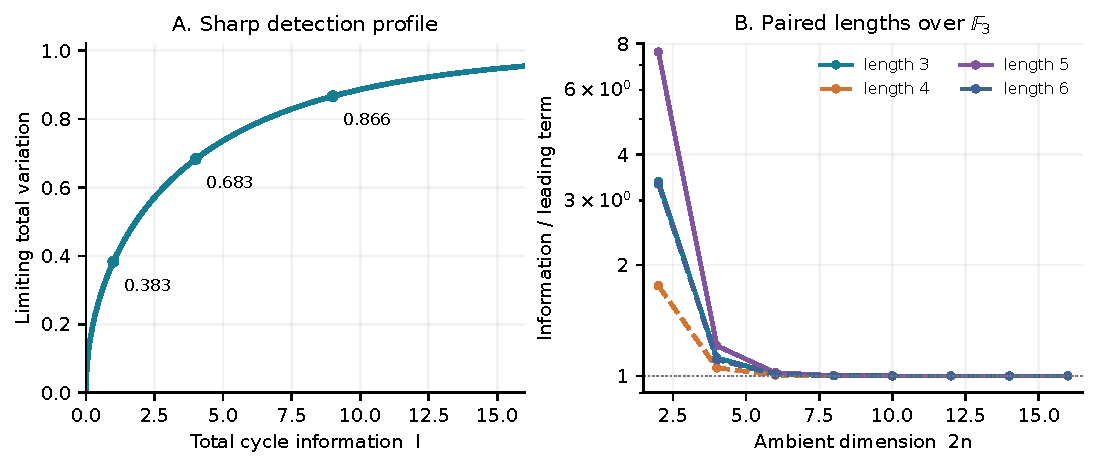
\includegraphics[width=.98\linewidth]{figures/detection_profile.pdf}
}{}
\caption{The sharp detection profile and leading information shared by paired
cycle lengths. The smooth curve is the proved limit. Finite information values
are computed from the exact rational formulas.}
\label{fig:profile}
\end{figure}


\IfFileExists{sections/overlap.tex}{\section{A contrasting critical law for overlapping cycles}\label{sec:overlap}

Keep $V=\mathbb F_q^{2n}$, $N=q^{2n}$ and the nonzero-vector sampling model.
Let $2\le a\le2n$. Assign independent uniform nonzero vectors
$X_1,\ldots,X_a$ to the left part of $K_{a,m}$ and
$Z_1,\ldots,Z_m$ to the right part. Orient all edges from left to right and
observe the columns
\[
 Y_j=(\langle X_1,Z_j\rangle,\ldots,
       \langle X_a,Z_j\rangle)\in\mathbb F_q^a.
\]
Let $P_{a,m,N}$ be the actual law and let
$Q_{a,m,N}=(p_N^{\otimes a})^{\otimes m}$ be the law with independent
edges and the same one-edge marginal.

Define a probability measure on $\mathbb F_q^a$ by
\[
 \rho_{a,N}(y)=
 \begin{cases}
 (N-q^a)/(q^a(N-1)),&y=0,\\
 N/(q^a(N-1)),&y\ne0.
 \end{cases}
\]
Its zero mass is allowed to vanish at the finite endpoint $a=2n$.
Put
\[
 \alpha_{a,N}=\prod_{i=0}^{a-1}\frac{N-q^i}{N-1},\qquad
 \delta_{a,N}=1-\alpha_{a,N}.
\]

\begin{proposition}[Exact independent-anchor reduction]\label{prop:anchors}
The event $\mathcal E$ that the $a$ anchor vectors are linearly independent
has probability $\alpha_{a,N}$. Conditional on $\mathcal E$, the columns
$Y_1,\ldots,Y_m$ are independent with common law $\rho_{a,N}$.
Consequently,
\[
 d_{\mathrm{TV}}(P_{a,m,N},\rho_{a,N}^{\otimes m})
 \le\delta_{a,N}
 \le\frac{(q^a-1)/(q-1)-a}{N-1}.
\tag{A1}
\]
Both inequalities hold for every $m$.

\end{proposition}
\begin{proof}
After $i$ independent nonzero anchors, the span contains $q^i-1$ of the
$N-1$ possible next vectors. Multiplying the successive probabilities
proves the formula for $\alpha_{a,N}$. The elementary product inequality
$1-\prod_i(1-b_i)\le\sum_i b_i$ with
$b_i=(q^i-1)/(N-1)$ gives the second bound.

For each fixed independent anchor tuple, nondegeneracy of the alternating
form makes the linear map
\[
 T_X:V\longrightarrow\mathbb F_q^a,
 \qquad z\longmapsto(\langle X_i,z\rangle)_{i=1}^a
\]
surjective. Every fibre has $N/q^a$ elements. Removing the zero vector
removes one point from the zero fibre only, giving $\rho_{a,N}$.
The $Z_j$ are independent, and this conditional column law does not depend
on the particular independent anchor tuple. Integrating over all such
tuples therefore preserves the product law. The mixture decomposition
\[
 P_{a,m,N}=\alpha_{a,N}\rho_{a,N}^{\otimes m}
             +\delta_{a,N}\mathcal D_{a,m,N}
\]
for a probability measure $\mathcal D_{a,m,N}$ proves the first bound.
\end{proof}

\begin{lemma}[Conditional column information]\label{lem:anchor-info}
For fixed $a,q$ and $n\to\infty$, uniformly on $y\in\mathbb F_q^a$,
\[
 \frac{\rho_{a,N}(y)}{p_N^{\otimes a}(y)}
 =1+\frac{h_a(y)}N+O_{a,q}(N^{-2}),
 \qquad
 h_a(y)=\sum_{i=1}^a\kappa(y_i)-\bigl(q^a\mathbf1_{y=0}-1\bigr).
\tag{A2}
\]
Under independent uniform coordinates, this score has mean zero and
\[
 \mathbb E h_a^2=J_{a,q}:=q^a-1-a(q-1)>0.
\tag{A3}
\]
In particular,
\[
 \chi^2(\rho_{a,N}\Vert p_N^{\otimes a})
 =J_{a,q}N^{-2}+O_{a,q}(N^{-3}).
\tag{A4}
\]

\end{lemma}
\begin{proof}
For $z=\#\{i:y_i=0\}$ and $y\ne0$, the likelihood is exactly
\[
 (1-N^{-1})^{a-1}(1-q/N)^{-z}.
\]
For $y=0$ it is
\[
 (1-q^a/N)(1-N^{-1})^{a-1}(1-q/N)^{-a}.
\]
Expanding these finite rational functions proves (A2).
Under uniform coordinates, the variables $\kappa(y_i)$ are independent,
have mean zero, and have second moment $q-1$. Moreover,
\[
 q^a\mathbf1_{y=0}=\prod_{i=1}^a(1+\kappa(y_i)),
 \qquad
 h_a(y)=-\sum_{\substack{S\subseteq\{1,\ldots,a\}\\|S|\ge2}}
               \prod_{i\in S}\kappa(y_i).
\]
The summands are pairwise orthogonal in $L^2$ of uniform product measure.
Their squared norms sum to
$\sum_{s=2}^a\binom as(q-1)^s=q^a-1-a(q-1)$, proving (A3).
The actual reference measure $p_N^{\otimes a}$ differs pointwise from the
uniform measure by $O_{a,q}(N^{-1})$, and (A2) then proves (A4).

For finite calculations there is also the exact identity
\[
 1+\chi^2(\rho_{a,N}\Vert p_N^{\otimes a})
 =\frac{(N-1)^{a-2}}{(N-q)^a}
   \left[N^{2-a}(N-q+1)^a+q^a-2N\right].
\tag{A5}
\]
To verify it, write
$\rho_{a,N}(y)=c(1-q^aN^{-1}\mathbf1_{y=0})$ with
$c=N/[q^a(N-1)]$, and sum its squared density over the product reference.
The two necessary sums are
\[
 \sum_{b\in\mathbb F_q}\frac1{p_N(b)}
 =\frac{q^2(N-1)(N-q+1)}{N(N-q)},\qquad
 \frac1{p_N(0)^a}=\left(\frac{q(N-1)}{N-q}\right)^a.
\]
Substitution and cancellation give (A5).
\end{proof}

\begin{theorem}[The fixed-anchor critical profile]\label{thm:anchors}
Fix $q$ and $a\ge2$. Let $n\to\infty$ and let $m=m_n$ be arbitrary
positive integers. If
\[
 \frac{mJ_{a,q}}{N^2}\longrightarrow\tau\in[0,\infty],
\]
then
\[
 d_{\mathrm{TV}}(P_{a,m,N},Q_{a,m,N})
 \longrightarrow 2\Phi(\sqrt\tau/2)-1,
\tag{A6}
\]
with value $1$ at $\tau=\infty$.
\end{theorem}
\begin{proof}
Indeed, apply \cref{lem:lan} to
$\rho_{a,N}^{\otimes m}$ and $(p_N^{\otimes a})^{\otimes m}$, using
(A2)--(A4). The difference between their distance and the actual distance
is at most $\delta_{a,N}=O_{a,q}(N^{-1})$ by (A1) and the triangle
inequality. This error is uniform in $m$.
\end{proof}

\subsection{Many overlapping four-cycles with vanishing total variation}
Set $a=2$. Now
\[
 \delta_{2,N}=\frac{q-1}{N-1},\qquad
 \chi^2(\rho_{2,N}\Vert p_N^{\otimes2})
      =\frac{(q-1)^2}{(N-q)^2}.
\]
The exact product chi-square identity and Cauchy--Schwarz give
\[
 d_{\mathrm{TV}}(P_{2,m,N},Q_{2,m,N})
 \le\frac{q-1}{N-1}
 +\frac12\sqrt{\left(1+\frac{(q-1)^2}{(N-q)^2}\right)^m-1}.
\tag{A7}
\]
The graph $K_{2,m}$ has exactly $\binom m2$ simple four-cycles.
Each four-cycle marginal has chi-square divergence
\[
 v_{4,N}=(q-1)^2\left((N-q)^{-2}+(q-2)(N-1)^{-2}\right)
       \sim(q-1)^3N^{-2}.
\]
Choose any fixed $1<\beta<2$ and $m=\lfloor N^\beta\rfloor$.
Then (A7) tends to zero, while
\[
 \binom m2 v_{4,N}\sim\frac{(q-1)^3}{2}N^{2\beta-2}
 \longrightarrow\infty.
\tag{A8}
\]
Thus summing the information of overlapping cycle marginals does not give
the information of the whole observation. The exact cactus factorization
is an essential hypothesis of the cycle-count criterion.

\subsection{The full chi-square divergence can diverge exponentially too}
Fix $c\in\mathbb F_q^\times$, and let $E_c$ be the data event
$Y_{2j}=cY_{1j}$ for every $1\le j\le m$.
The latent event $X_2=cX_1$ has probability $1/(N-1)$ and forces $E_c$,
so $P_{2,m,N}(E_c)\ge1/(N-1)$.
Under the independent-edge law,
\[
 Q_{2,m,N}(E_c)=s_N^m,\qquad
 s_N=p_N(0)^2+(q-1)p_N(1)^2
    =\frac1q+\frac{q-1}{q(N-1)^2}.
\]
Since $1+\chi^2(P\Vert Q)=\sum_y P(y)^2/Q(y)$, applying
Cauchy--Schwarz on $E_c$ gives the exact lower bound
\[
 1+\chi^2(P_{2,m,N}\Vert Q_{2,m,N})
 \ge\frac1{(N-1)^2s_N^m}.
\tag{A9}
\]
For the same $m=\lfloor N^\beta\rfloor$, $1<\beta<2$,
\[
 \log(1+\chi^2(P_{2,m,N}\Vert Q_{2,m,N}))
 \ge m\log q-2\log(N-1)-O_q(m/N^2)
 \longrightarrow\infty,
\]
even though the total variation distance tends to zero.
The rare dependent-anchor configurations therefore have negligible total
probability and arbitrarily large likelihood ratios. This explicitly
explains why a direct second-moment bound for the original mixture may be
very poor, whereas conditioning on anchor independence identifies its
correct testing profile.
}{}
\section{Reproducibility, proof status, and comparison}\label{sec:provenance}

\subsection{Independent computations}
The archive contains complete \LaTeX\ sources and compiled PDFs, an exact rational
law calculator, independent finite-field enumeration, recorded results, and a
formalization plan. The calculator groups labels by sufficient statistics.
The independent checker instead constructs actual vector assignments and counts
their edge observations; it does not use a proposed formula to generate those
counts. It includes the extension field
$\F_4=\F_2[z]/(z^2+z+1)$.

The direct enumeration verified:
\begin{itemize}
\item $1{,}745{,}891$ nonzero-vector assignments across $16$ cycle cases, four
cactus cases, and five tree cases;
\item all $1{,}976$ resulting cycle label probabilities, their exact total
variation and chi-square divergences;
\item $608$ proper cycle-edge subsets, giving $11{,}614$ marginal equalities;
\item six additive-character inversions for even-cycle resonance.
\end{itemize}
The fields were $\F_2,\F_3,\F_4,\F_5$, and ambient dimensions were two or four.
All comparisons passed. A separate $432$-case arithmetic check compared the
grouped likelihoods with the closed formulas for
$q\in\{2,3,4,5,7,8,9,16,25\}$ and several dimensions and cycle lengths.

A further twenty complete-bipartite cases enumerate $4{,}094{,}368$ assignments and check $7{,}382$ full label probabilities. Thus the two graph verifiers together cover $5{,}840{,}259$ actual assignments. They also check sixteen limiting-score variances by exact summation over $5{,}680$ label vectors.

These finite checks are regression evidence, not the proof for arbitrary
$q,n$. The proof is the character calculation, exact finite summation,
block factorization, and probability-limit argument. No Monte Carlo
approximation is used to establish an exact identity or the normal limit.
Further companion checks, where included, are reported separately in their
own files so their scope is not conflated with these totals.

\subsection{Source audit and novelty scope}
The pinned repository distinguishes unconditional results, uses of Dirichlet
GRH, and reductions whose target estimates remain open. Its README describes
the large article as a merge of reports, not an independent verification of
every claim \cite{ProveItReadme}. The vendored upstream is pinned at
\texttt{72fead102f663d5c7a407964a13dc0cf9d977207}; this work did not rerun that
development's kernel checks. Our new theorems do not require them.

The principal mathematical input from the repository is a method: evaluate
finite-field Fourier transforms using bilinear orthogonality, then retain
the structured information needed to compute the full law. The identity
$F_sF_t=NP_{s/t}-J$ makes this transfer exact on graph cycles. We prove it
directly. Consequently a revision elsewhere in the analytic corpus would not
affect these results.

Related primary literature includes cycle counts for distance and dot-product
graphs \cite{IJM}, extensions to general nondegenerate bilinear forms
\cite{Bright}, classical finite symplectic graph theory \cite{TangWan}, and
topology-dependent distinguishability for real masked Wishart matrices
\cite{BBH}. Those works establish relevant background. Special fixed-label cycle
counts can also follow from known graph spectra. The contribution here is the
complete labelled finite-field law relative to the product of its true
marginals, followed by the exact critical profile and explicit overlapping-cycle
contrast. We did not find this combined statement in the inspected repository
or the specifically reviewed references. This is a scoped novelty assessment,
not a proof of worldwide bibliographic priority.

The results have not been encoded and checked in Lean. The formalization plan
separates finite algebra from probability limits and states what needs formal
proof. It contains no placeholder presented as a verified theorem.

\subsection{Scope and remaining questions}
The cactus hypothesis is substantive. Our complete-bipartite calculation handles
one family of overlapping cycles, but does not give a general answer for every
graph. The bounded cycle-length hypothesis controls all likelihood increments
uniformly. If the lengths grow with $n$, further estimates are needed.
Nonuniform vector laws, zero vectors, projective sampling, and distinctness
constraints on graph-vertex vectors are different models.

A natural next problem is to determine the information contributed by overlapping
cycles in more general graphs. The complete-bipartite example shows that adding
the individual cycle chi-square values can fail drastically. The unconditional
graph likelihood can have extremely rare, very large values even when its total
variation distance tends to zero. Any wider theorem must account for this effect.

The archive also includes a separate companion theorem about the full
cross-pairing matrix of arbitrarily many prescribed small frames. Its assumptions,
proof, comparison with earlier rank-universality literature, and numerical
checks are self-contained in that paper.


\appendix
\section{Grouped laws for exact calculation}\label{app:groups}
The following formulas specify a small sufficient-statistic experiment.
They are implemented with rational arithmetic in \texttt{code/cycle\_laws.py}.
Let $z$ be the number of zero labels, and set $p_0=p_N(0)$,
$p_1=p_N(a)$ for any $a\ne0$.

For odd $\ell=2r+1$, the independent-model mass of the group $z$ is
\[
Q_z=\binom{\ell}{z}p_0^z((q-1)p_1)^{\ell-z},
\]
and its likelihood ratio is
\[
L_z=1+N^{-r}
\left(\frac{(q-1)N}{N-q}\right)^z(-1)^{\ell-z}.
\]
Its symplectic mass is $Q_zL_z$.

For even $\ell=2k$, each group with $z\ge1$ has the same $Q_z$ and
\[
L_z
=1+\frac{N^k(N-q)(q-1)^{z-1}(-1)^z}
{(N-q)^z N^{\ell-z}}.
\]
When $z=0$, split into resonant and nonresonant groups:
\[
Q_{\rm res}=(q-1)^{\ell-1}p_1^\ell,\qquad
Q_{\rm non}=(q-2)(q-1)^{\ell-1}p_1^\ell,
\]
\[
L_{\rm res}
=1+N^{-k}\frac{N-q+(q-2)(N-1)q^k}{q-1},\qquad
L_{\rm non}
=1+N^{-k}\frac{N-q-(N-1)q^k}{q-1}.
\]
Omit the nonresonant group for $q=2$. Some symplectic masses can vanish for
small parameters; the formulas remain valid.

\section{Proof dependencies and formalization boundary}
The argument has the following dependencies:
\begin{enumerate}
\item Nondegeneracy of the alternating form gives the one-edge law.
\item Leaf removal gives forest independence.
\item Additive-character orthogonality gives $F_sF_t=NP_{s/t}-J$.
\item The cyclic trace gives the complete cycle Fourier law.
\item Additive inversion and one elementary Gauss-sum identity give the
pointwise cycle law.
\item Finite sums give exact total variation and chi-square values.
\item Symplectic transitivity and the block-cut tree give cactus factorization.
\item Taylor expansion, independence, and a central limit theorem give the
critical profile.
\item Conditioning on independent anchors gives the complete-bipartite
comparison, and the same product lemma gives its distinct critical scale.
\end{enumerate}
No step imports RH, GRH, an unproved finite-field estimate, or a numerical
extrapolation. A Lean formalization would need to implement the finite
probability spaces, the character matrices and their invariant subspaces,
the graph decomposition, and the triangular-array limit theorem.
The accompanying \texttt{FORMALIZATION.txt} gives more precise interfaces.


\begin{thebibliography}{99}
\raggedright
\bibitem{ProveItSpn}
V. Reshetnikov, ProveIt repository,
\emph{Beyond the Riemann hypothesis for Dirichlet L-functions:
consequences, transfers and limits}, section
\emph{Spanning, frames, auxiliary characters and matrix statistics}.
Pinned snapshot \texttt{00cadb961bbe77c74e5d082c4948f8884d58a970},
27 November 2026.
\url{https://github.com/VladimirReshetnikov/ProveIt/blob/00cadb961bbe77c74e5d082c4948f8884d58a970/Analysis/GeneralizedRiemannHypothesis/Article/sections/spn.tex}.

\bibitem{ProveItSrc}
Same repository and snapshot, section \emph{The source theorem and its
transferable mechanism}, \texttt{Article/sections/src.tex}.
\url{https://github.com/VladimirReshetnikov/ProveIt/blob/00cadb961bbe77c74e5d082c4948f8884d58a970/Analysis/GeneralizedRiemannHypothesis/Article/sections/src.tex}.

\bibitem{ProveItTwo}
Same repository and snapshot, \emph{Two open questions from the ProveIt GRH
article}, symplectic component.
\url{https://github.com/VladimirReshetnikov/ProveIt/blob/00cadb961bbe77c74e5d082c4948f8884d58a970/Analysis/GeneralizedRiemannHypothesis/Research/grh-two-open-questions/symplectic/symplectic.tex}.

\bibitem{ProveItRect}
Same repository and snapshot, \emph{Uniform rank and joint-defect laws for
rectangular symplectic blocks}.
\url{https://github.com/VladimirReshetnikov/ProveIt/tree/00cadb961bbe77c74e5d082c4948f8884d58a970/Analysis/GeneralizedRiemannHypothesis/Research/rectangular_symplectic_blocks}.

\bibitem{ProveItReadme}
Same repository and snapshot, article README and project README.
\url{https://github.com/VladimirReshetnikov/ProveIt/blob/00cadb961bbe77c74e5d082c4948f8884d58a970/Analysis/GeneralizedRiemannHypothesis/Article/README.md}.

\bibitem{IJM}
A. Iosevich, G. Jardine and B. McDonald,
\emph{Cycles of arbitrary length in distance graphs on $\F_q^d$},
arXiv:2101.00748 (2021).
\url{https://arxiv.org/abs/2101.00748}.

\bibitem{Bright}
P. Bright, X. Fang, B. Heritage, A. Iosevich, T. Jiang, H. Parshall and M. Sun,
\emph{Generalized point configurations in $\F_q^d$},
arXiv:2308.10853 (2023).
\url{https://arxiv.org/abs/2308.10853}.

\bibitem{TangWan}
Z. Tang and Z.-X. Wan,
\emph{Symplectic graphs and their automorphisms},
European Journal of Combinatorics \textbf{27} (2006), 38--50.
\url{https://doi.org/10.1016/j.ejc.2004.08.002}.

\bibitem{BBH}
M. Brennan, G. Bresler and B. Huang,
\emph{De Finetti-Style Results for Wishart Matrices: Combinatorial Structure
and Phase Transitions}, arXiv:2103.14011 (2021).
\url{https://arxiv.org/abs/2103.14011}.
\end{thebibliography}


\end{document}

